\documentclass[aspectratio=169,11pt]{beamer}

\usetheme{metropolis}
\usepackage{amsmath,amssymb}
\usepackage{siunitx}
\usepackage{tikz}
\usetikzlibrary{decorations.pathmorphing,arrows.meta,calc,patterns}
\usepackage{pgfplots}
\pgfplotsset{compat=1.18}

\newcommand{\vect}[1]{\mathbf{#1}}
\newcommand{\uu}{\vect{u}}
\newcommand{\ww}{\vect{w}}
\newcommand{\ez}{\vect{e}_z}

\definecolor{sand}{HTML}{E0A030}
\definecolor{bolt}{HTML}{C0392B}
\definecolor{modeblue}{HTML}{2E6FB7}

\tikzset{
  spring/.style={decorate,decoration={zigzag,segment length=4pt,amplitude=3pt,pre length=3pt,post length=3pt}},
  mass/.style={draw,fill=modeblue!25,minimum size=7mm,rounded corners=1pt},
}

\title{Why Sand Draws Patterns}
\subtitle{The mathematics behind the Chladni plate}
\author{Mauro Morini}
\institute{University of Basel}
\date{}

\begin{document}

\maketitle

% ---------------------------------------------------------------------------
\section{The experiment}

\begin{frame}{The Chladni experiment}
  \begin{columns}[c]
    \begin{column}{0.5\textwidth}
      \begin{itemize}
        \item A thin metal plate is screwed onto a \textcolor{bolt}{bolt} in its center.
        \item A shaker moves the bolt up and down, a few hundred times per second.
        \item Sand sprinkled on top jumps around \dots
        \item \dots and collects along lines: a \alert{Chladni figure}.
        \item Each frequency gives a different figure.
      \end{itemize}
    \end{column}
    \begin{column}{0.48\textwidth}
      \centering
      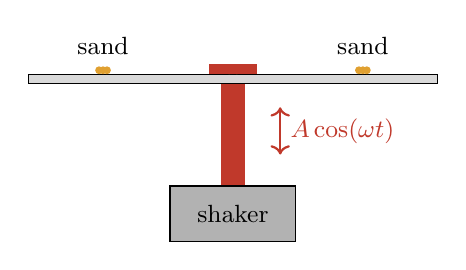
\begin{tikzpicture}[scale=1.0]
        % plate
        \fill[gray!30] (-2.6,0) rectangle (2.6,0.12);
        \draw (-2.6,0) rectangle (2.6,0.12);
        % sand grains
        \foreach \x in {-1.7,-1.6,-1.65,1.6,1.7,1.65,-0.05,0.05}
          \fill[sand] (\x,0.17) circle (0.05);
        % bolt
        \fill[bolt] (-0.15,-1.3) rectangle (0.15,0);
        \fill[bolt] (-0.3,0.12) rectangle (0.3,0.25);
        % shaker
        \draw[fill=gray!60] (-0.8,-2.0) rectangle (0.8,-1.3);
        \node at (0,-1.65) {\small shaker};
        \draw[<->,thick,bolt] (0.6,-0.9) -- (0.6,-0.3) node[right,midway] {\small $A\cos(\omega t)$};
        \node[above] at (-1.65,0.25) {\small sand};
        \node[above] at (1.65,0.25) {\small sand};
      \end{tikzpicture}
    \end{column}
  \end{columns}
\end{frame}

\begin{frame}{What we want to compute}
  Every point of the plate moves a little bit. We describe this by the
  \alert{displacement}, a vector with three components:
  \[
    \uu(x,y,z,t) =
    \begin{pmatrix} u_x \\ u_y \\ u_z \end{pmatrix}
    \quad
    \begin{array}{l}
      \leftarrow \text{sideways } (x) \\
      \leftarrow \text{sideways } (y) \\
      \leftarrow \text{up / down } (z)
    \end{array}
  \]
  \begin{itemize}
    \item $u_z$ is the important one: it throws the sand up.
    \item $u_x, u_y$ are small: when a thin plate bends, its top and bottom shift a little sideways.
    \item Sizes: the plate is \SI{24}{cm} wide and \SI{1}{mm} thick, but it only moves by
          \alert{micrometers}.
  \end{itemize}
  \medskip
  \textbf{Questions:} At which frequencies does the plate vibrate strongly?
  Which shape does it have? Where does the sand stop?
\end{frame}

% ---------------------------------------------------------------------------
\section{From Newton to an equation}

\begin{frame}{Idea: cut the plate into small pieces}
  \begin{columns}[c]
    \begin{column}{0.55\textwidth}
      Think of the plate as many small \alert{masses} connected by \alert{springs}.
      \medskip

      For each piece $i$, Newton's law $m a = F$ says
      \[
        m\,\ddot u_i = \underbrace{k(u_{i+1}-u_i)}_{\text{right spring}}
                     + \underbrace{k(u_{i-1}-u_i)}_{\text{left spring}}
      \]
      ($\ddot u_i$ = acceleration = second time derivative.)
      \medskip

      \textbf{Important:} a spring only feels the \alert{difference} of the two ends,
      $u_{i+1}-u_i$, i.e.\ how much it is stretched.
    \end{column}
    \begin{column}{0.43\textwidth}
      \centering
      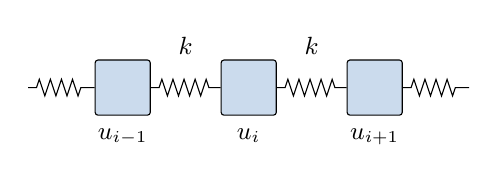
\begin{tikzpicture}
        \node[mass] (m1) at (0,0) {};
        \node[mass] (m2) at (1.6,0) {};
        \node[mass] (m3) at (3.2,0) {};
        \draw[spring] (-1.2,0) -- (m1);
        \draw[spring] (m1) -- (m2);
        \draw[spring] (m2) -- (m3);
        \draw[spring] (m3) -- (4.4,0);
        \node[below=4mm] at (m1) {\small $u_{i-1}$};
        \node[below=4mm] at (m2) {\small $u_i$};
        \node[below=4mm] at (m3) {\small $u_{i+1}$};
        \node[above=3mm] at ($(m1)!0.5!(m2)$) {\small $k$};
        \node[above=3mm] at ($(m2)!0.5!(m3)$) {\small $k$};
      \end{tikzpicture}
      \medskip

      {\small The real computation uses $\sim 10^5$ pieces in 3D
      (the \emph{finite element method}), but the idea is the same.}
    \end{column}
  \end{columns}
\end{frame}

\begin{frame}{All pieces at once: a matrix equation}
  Collect all displacements in one long vector $\uu = (u_1, u_2, \dots, u_N)$.
  All the Newton equations together read
  \[
    \boxed{\;M\,\ddot\uu + K\,\uu = \vect{0}\;}
  \]
  \begin{itemize}
    \item $M$ = \alert{mass matrix}: how heavy each piece is.
    \item $K$ = \alert{stiffness matrix}: how the springs connect the pieces.
  \end{itemize}
  \medskip
  Example with 2 masses between two walls:
  \[
    \underbrace{\begin{pmatrix} m & 0 \\ 0 & m \end{pmatrix}}_{M}
    \begin{pmatrix} \ddot u_1 \\ \ddot u_2 \end{pmatrix}
    +
    \underbrace{\begin{pmatrix} 2k & -k \\ -k & 2k \end{pmatrix}}_{K}
    \begin{pmatrix} u_1 \\ u_2 \end{pmatrix}
    = \begin{pmatrix} 0 \\ 0 \end{pmatrix}
  \]
\end{frame}

\begin{frame}{Vibrating at one frequency}
  We look for motions where every piece swings \alert{in sync} with the same frequency $f$:
  \[
    \uu(t) = \hat\uu\,\cos(\omega t), \qquad \omega = 2\pi f .
  \]
  $\hat\uu$ is the \alert{shape} (how far each piece swings), $\cos(\omega t)$ is the rhythm.
  \medskip

  Since $\ddot\uu = -\omega^2\,\hat\uu\cos(\omega t)$, the equation becomes
  \[
    -\omega^2 M\hat\uu\cos(\omega t) + K\hat\uu\cos(\omega t) = \vect 0
    \quad\Longrightarrow\quad
    \boxed{\;K\,\hat\uu = \omega^2 M\,\hat\uu\;}
  \]
  This is an \alert{eigenvalue problem}:
  \begin{itemize}
    \item only special values $\omega_1, \omega_2, \dots$ (the \emph{eigenfrequencies}) work,
    \item each comes with a special shape $\boldsymbol\varphi_1, \boldsymbol\varphi_2, \dots$
          (the \emph{eigenmodes}).
  \end{itemize}
\end{frame}

\begin{frame}{Example: two masses}
  \begin{columns}[c]
    \begin{column}{0.55\textwidth}
      Solving $K\hat\uu = \omega^2 M\hat\uu$ for the 2-mass example gives:
      \medskip

      \textbf{Mode 1:} $\omega_1^2 = k/m$, \quad $\boldsymbol\varphi_1 = (1,\;1)$\\
      {\small both masses move together}
      \medskip

      \textbf{Mode 2:} $\omega_2^2 = 3k/m$, \quad $\boldsymbol\varphi_2 = (1,\,-1)$\\
      {\small masses move against each other, faster}
      \medskip

      \alert{Check mode 1:}
      $K\boldsymbol\varphi_1 = (2k-k,\; -k+2k) = k\,(1,1) = \tfrac{k}{m}\, M\boldsymbol\varphi_1$ \checkmark
    \end{column}
    \begin{column}{0.43\textwidth}
      \centering
      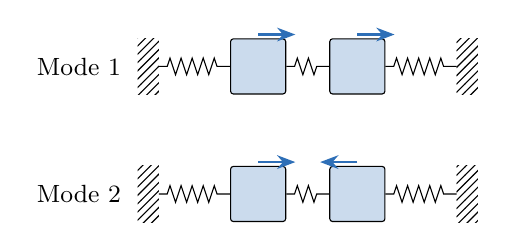
\begin{tikzpicture}[scale=0.9]
        \foreach \y/\a/\b/\lab in {0/0.35/0.35/{Mode 1}, -1.8/0.35/-0.35/{Mode 2}} {
          \fill[pattern=north east lines] (-0.3,\y-0.4) rectangle (0,\y+0.4);
          \fill[pattern=north east lines] (4.2,\y-0.4) rectangle (4.5,\y+0.4);
          \node[mass] (a) at (1.4,\y) {};
          \node[mass] (b) at (2.8,\y) {};
          \draw[spring] (0,\y) -- (a);
          \draw[spring] (a) -- (b);
          \draw[spring] (b) -- (4.2,\y);
          \draw[-{Stealth},thick,modeblue] (1.4,\y+0.45) -- ++(\a*1.5,0);
          \draw[-{Stealth},thick,modeblue] (2.8,\y+0.45) -- ++(\b*1.5,0);
          \node[left] at (-0.4,\y) {\small \lab};
        }
      \end{tikzpicture}
    \end{column}
  \end{columns}
  \medskip
  \alert{Note:} $2\boldsymbol\varphi_1 = (2,2)$ is also a solution. The eigenvalue problem
  gives the \emph{shape}, but \alert{not the size} of the motion.
\end{frame}

% ---------------------------------------------------------------------------
\section{Boundary conditions}

\begin{frame}{What happens at the edges and at the bolt?}
  The equation $M\ddot\uu + K\uu = \vect 0$ holds \emph{inside} the plate.
  We also have to say what happens at its border: \alert{boundary conditions}.
  \bigskip

  \begin{columns}[t]
    \begin{column}{0.48\textwidth}
      \textbf{Outer edges: free}
      \begin{itemize}
        \item Nothing holds or pushes the edges.
        \item Mathematically: the force on the edge surface is zero.
        \item In the spring picture: the last mass has a spring on one side only.
      \end{itemize}
    \end{column}
    \begin{column}{0.48\textwidth}
      \textbf{Bolt: clamped}
      \begin{itemize}
        \item The plate is screwed tightly to the bolt.
        \item In the eigenvalue problem we set
          \[
            \hat\uu = \begin{pmatrix} 0\\0\\0 \end{pmatrix} \text{ on the bolt.}
          \]
        \item All three components: no sliding, no lifting.
      \end{itemize}
    \end{column}
  \end{columns}
\end{frame}

\begin{frame}[standout]
  But wait \dots\\[1em]
  the shaker moves the bolt up and down!\\[1em]
  Why is $\hat\uu = \vect 0$ on the bolt correct?
\end{frame}

\begin{frame}{The real condition on the bolt}
  The shaker moves the bolt only vertically, with a small amplitude $A$
  (about \SI{1}{\micro m}):
  \[
    \uu = \begin{pmatrix} 0 \\ 0 \\ A\cos(\omega t) \end{pmatrix}
    \quad \text{on the bolt.}
  \]
  \begin{itemize}
    \item $x$ and $y$: $0$, because the bolt does not move sideways.
    \item $z$: $A\cos(\omega t)$, the up-and-down motion of the shaker.
  \end{itemize}
  \medskip
  This is \emph{not} zero. So the plate really does move at the bolt.
  \medskip

  \alert{Trick:} look at the plate from the point of view of the bolt.
\end{frame}

\begin{frame}{Trick: ride along with the bolt}
  \begin{columns}[c]
    \begin{column}{0.58\textwidth}
      Sit in an elevator that moves with the bolt. Split the motion:
      \[
        \uu \;=\; \underbrace{A\cos(\omega t)\,\ez}_{\substack{\text{whole plate moves}\\\text{with the bolt}}}
        \;+\; \underbrace{\ww}_{\substack{\text{bending, seen}\\\text{from the elevator}}}
      \]
      with $\ez = (0,0,1)$. Component by component:
      \[
        u_x = w_x,\quad u_y = w_y,\quad u_z = A\cos(\omega t) + w_z .
      \]
      On the bolt $\uu = (0,0,A\cos\omega t)$, therefore
      $\boxed{\;\ww = (0,0,0) \text{ on the bolt}\;}$
    \end{column}
    \begin{column}{0.40\textwidth}
      \centering
      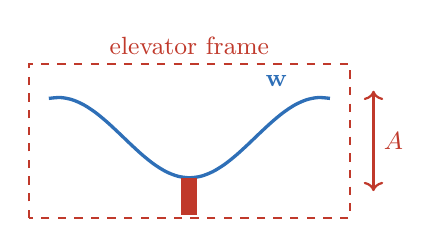
\begin{tikzpicture}[scale=0.85]
        % elevator frame
        \draw[thick,dashed,bolt] (-2.4,-0.9) rectangle (2.4,1.4);
        \node[bolt,above] at (0,1.4) {\small elevator frame};
        \draw[<->,thick,bolt] (2.75,-0.5) -- (2.75,1.0) node[midway,right] {\small $A$};
        % bent plate
        \draw[very thick,modeblue] plot[smooth,domain=-2.1:2.1] (\x,{0.6*(1-cos(deg(1.6*abs(\x))))-0.3});
        \fill[bolt] (-0.12,-0.85) rectangle (0.12,-0.3);
        \node[modeblue] at (1.3,1.15) {\small $\ww$};
      \end{tikzpicture}
      \medskip

      {\small From inside the elevator the bolt does not move.}
    \end{column}
  \end{columns}
\end{frame}

\begin{frame}{The springs do not notice the elevator}
  What is the equation for $\ww$? Put $\uu = A\cos(\omega t)\,\vect r + \ww$ into
  $M\ddot\uu + K\uu = \vect 0$.\\
  Here $\vect r = (0,0,1,\;0,0,1,\;\dots)$ means ``every piece moves up by 1''.
  \medskip

  \textbf{Key fact:} if every piece moves up by the same amount, no spring is stretched:
  \[
    u_{i+1} - u_i \text{ does not change}
    \quad\Longrightarrow\quad
    K\vect r = \vect 0 .
  \]
  So only the acceleration of the elevator remains:
  \[
    M\ddot\ww + K\ww = \underbrace{\omega^2 A\cos(\omega t)\, M\vect r}_{\text{shaking force}}
    \qquad\text{and}\qquad \ww = \vect 0 \text{ on the bolt.}
  \]
  \alert{Inside the elevator}, the bolt is fixed and every piece feels an extra up-and-down
  force, just like you are pushed into your seat when a bus brakes.
\end{frame}

\begin{frame}{Pushing a swing: resonance}
  \begin{columns}[c]
    \begin{column}{0.52\textwidth}
      Near $\omega_k$, $\ww \approx c\,\boldsymbol\varphi_k\cos(\omega t)$, where
      $\boldsymbol\varphi_k$ is a mode of the \alert{clamped} plate. One finds
      \[
        c = \frac{\omega^2\,A\,p_k}{\omega_k^2 - \omega^2}
      \]
      \begin{itemize}
        \item $A$: how hard we shake.
        \item $p_k$: how well the shaking ``fits'' mode $k$.
        \item $\omega \to \omega_k$: denominator $\to 0$,
              motion becomes \alert{huge}.
      \end{itemize}
      Friction keeps it finite: a few hundred times $A$.
    \end{column}
    \begin{column}{0.46\textwidth}
      \centering
      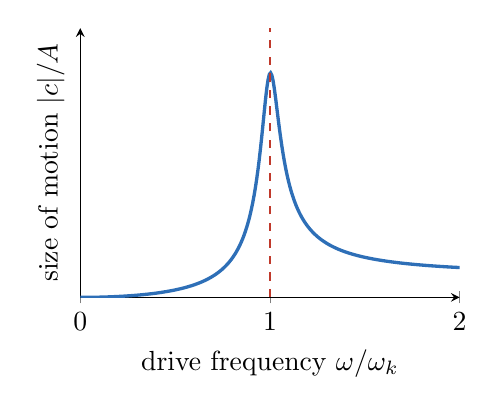
\begin{tikzpicture}
        \begin{axis}[
            width=6.4cm, height=5cm,
            xlabel={drive frequency $\omega/\omega_k$},
            ylabel={size of motion $|c|/A$},
            xmin=0, xmax=2, ymin=0, ymax=12,
            ytick=\empty, xtick={0,1,2},
            axis lines=left,
          ]
          \addplot[very thick,modeblue,domain=0:2,samples=300]
            {x^2/sqrt((1-x^2)^2 + (0.1*x)^2)};
          \draw[dashed,bolt] (axis cs:1,0) -- (axis cs:1,12);
        \end{axis}
      \end{tikzpicture}
    \end{column}
  \end{columns}
\end{frame}

\begin{frame}{So why is $\hat\uu = \vect 0$ on the bolt correct?}
  \begin{enumerate}
    \item Seen from the bolt, the plate bends with $\ww$, and $\ww = \vect 0$ on the bolt.
    \item $\ww$ becomes large exactly when $\omega$ is an eigenfrequency of the
          \alert{clamped} plate.
    \item Then $\ww$ has the shape of the clamped eigenmode $\boldsymbol\varphi_k$.
  \end{enumerate}
  \medskip
  So the clamped problem gives the \alert{right frequencies and the right shapes}.
  \medskip

  \textbf{It does not mean the plate is still:}
  \begin{itemize}
    \item $\vect 0$ only on the small bolt, and only \emph{relative to the bolt}.
    \item The size of the motion comes from $A$ and from resonance,
          not from the eigenvalue problem.
  \end{itemize}
\end{frame}

% ---------------------------------------------------------------------------
\section{Where does the sand go?}

\begin{frame}{The complete motion}
  Back in the lab (outside the elevator), near the resonance $\omega\approx\omega_k$:
  \[
    \uu(t) \approx \hat\uu\cos(\omega t),\qquad
    \hat\uu =
    \begin{pmatrix} \hat u_x \\ \hat u_y \\ \hat u_z \end{pmatrix}
    \approx
    \begin{pmatrix} c\,\varphi_{k,x} \\ c\,\varphi_{k,y} \\ A + c\,\varphi_{k,z} \end{pmatrix}
  \]
  \begin{itemize}
    \item On the bolt $\boldsymbol\varphi_k = \vect 0$, so $\hat\uu = (0,0,A)$:
          the bolt moves with the shaker. \checkmark
    \item Elsewhere $|c\,\varphi_{k,z}|$ is hundreds of times larger than $A$.
    \item $\hat u_x, \hat u_y$ are small sideways motions; sand mostly reacts to $\hat u_z$.
  \end{itemize}
\end{frame}

\begin{frame}{Sand stops where the plate does not move up and down}
  A grain is thrown up when the plate accelerates downward faster than gravity:
  \[
    |\hat u_z|\,\omega^2 > g \approx \SI{9.81}{m/s^2}.
  \]
  \begin{itemize}
    \item At the bolt: $|\hat u_z| = A$. With $A = \SI{1}{\micro m}$ and $f = \SI{1000}{Hz}$:
      $A\omega^2 \approx \SI{39}{m/s^2} \approx 4g$. The sand still hops!
    \item Far from the lines: much stronger, sand is thrown away.
    \item The sand only comes to rest where $\hat u_z \approx 0$:
      \[
        A + c\,\varphi_{k,z} = 0
        \quad\Longleftrightarrow\quad
        \varphi_{k,z} = -\frac{A}{c} \approx 0 .
      \]
  \end{itemize}
  \alert{Result:} the sand lines are (almost exactly) the lines where the clamped eigenmode
  $\varphi_{k,z}$ is zero, the \emph{nodal lines}.
\end{frame}

\begin{frame}{Computed Chladni figures}
  \centering
  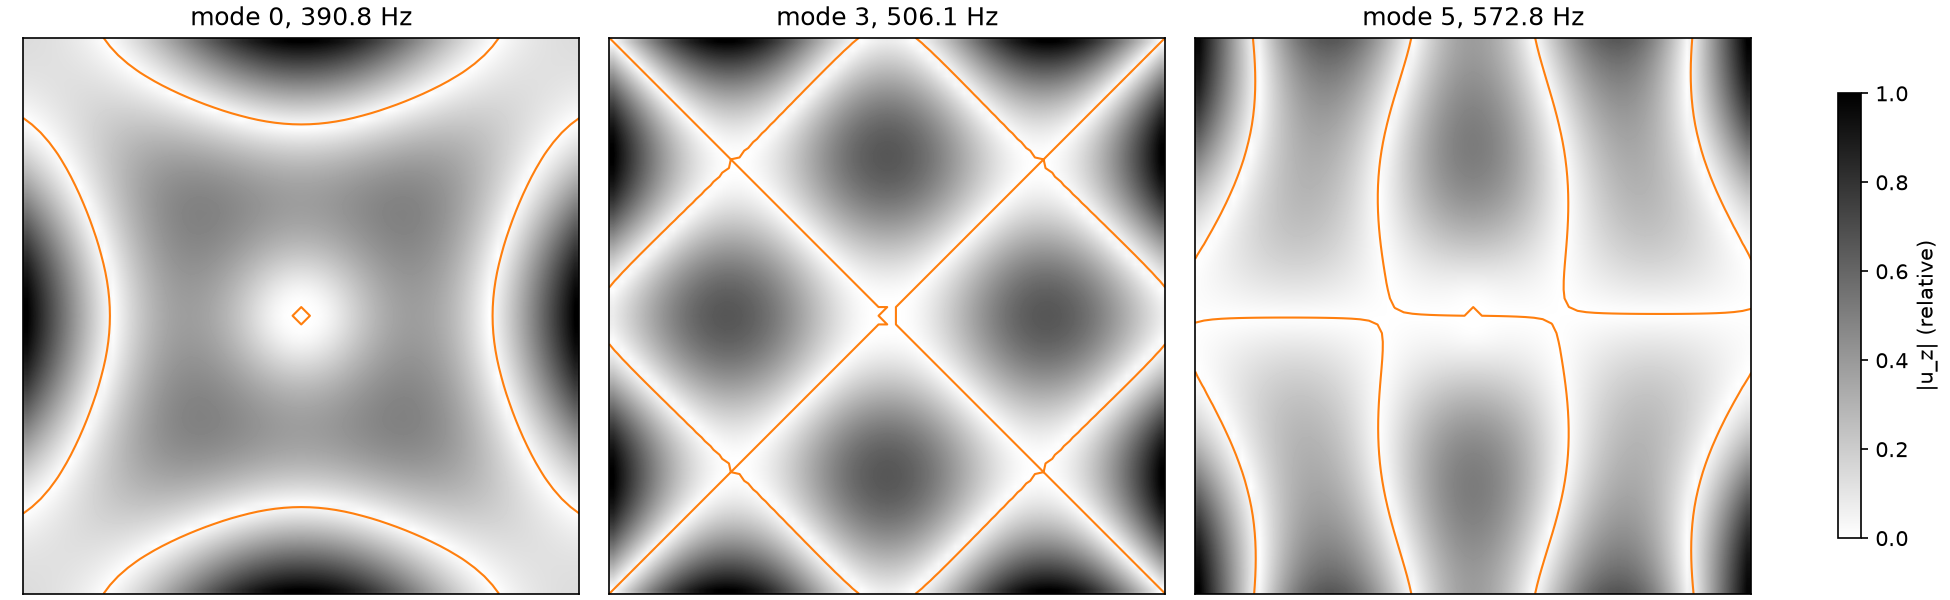
\includegraphics[width=\textwidth]{figures/patterns.png}
  \medskip

  {\small Aluminium plate, \SI{24}{cm} $\times$ \SI{24}{cm} $\times$ \SI{1}{mm}, clamped bolt
  of radius \SI{5}{mm}. Bright: plate at rest (sand). Orange: nodal lines $\varphi_{k,z}=0$.\\
  The small orange ring in the center of mode 0 is the clamped bolt.}
\end{frame}

% ---------------------------------------------------------------------------
\section{Summary}

\begin{frame}{Summary}
  \begin{enumerate}
    \item Newton's law for many small pieces: $M\ddot\uu + K\uu = \vect 0$.
    \item One frequency: $K\hat\uu = \omega^2 M\hat\uu$, an eigenvalue problem.
          It gives \alert{frequencies} and \alert{shapes}, not sizes.
    \item Boundary conditions: free edges, and $\hat\uu = (0,0,0)$ on the bolt.
    \item The bolt really moves by $(0,0,A\cos\omega t)$. Seen from the bolt, the plate
          is clamped and pushed by a shaking force. Springs do not feel a common shift
          ($K\vect r = \vect 0$).
    \item Near an eigenfrequency the plate resonates; the size of the motion is set by $A$.
    \item Sand collects where $\hat u_z = A + c\,\varphi_{k,z} = 0$, i.e.\ (almost)
          on the nodal lines of the clamped eigenmode.
  \end{enumerate}
\end{frame}

\end{document}
